% 图 5.15 (a) 螺旋磁有序（逐层旋转 30 度的磁矩堆叠）(b) J1-J2 相图（铁磁/反铁磁/螺旋）
\documentclass[tikz,border=5pt]{standalone}
\usetikzlibrary{arrows.meta,calc}
\usepackage{amsmath}
\usepackage{bm}
\usepackage{fontspec}
\setmainfont{Times New Roman}
\begin{document}
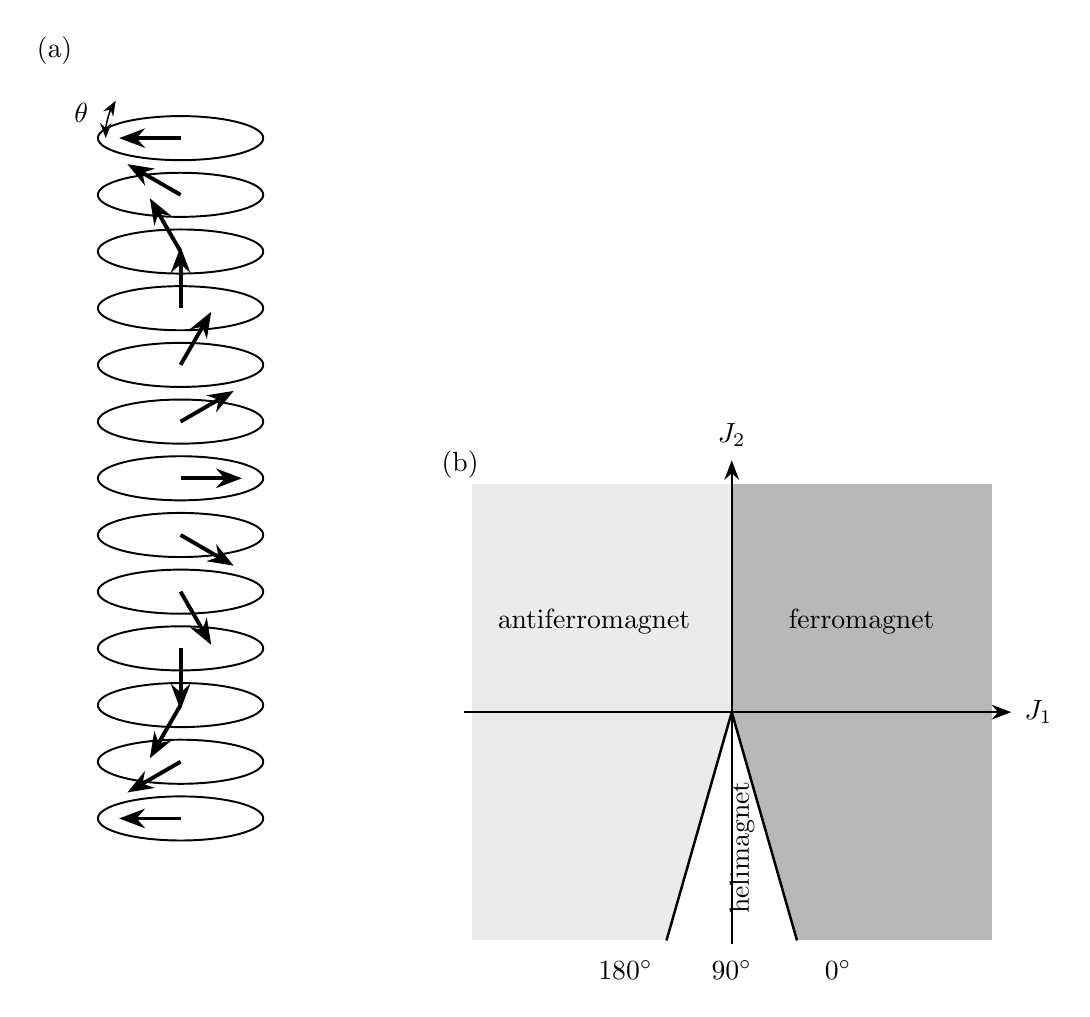
\begin{tikzpicture}[line width=0.8pt,>=Stealth]
% ---------- (a) helix: 13 layers, angle step 30 deg CCW going up ----------
\begin{scope}[shift={(0,0)}]
  \foreach \i in {0,...,12}{
    \pgfmathsetmacro{\yy}{\i*0.72}
    \pgfmathsetmacro{\aa}{180+\i*30}
    \draw[line width=0.7] (0,\yy) ellipse [x radius=1.05, y radius=0.28];
    \draw[->,line width=1.4] (0,\yy) -- ++(\aa:0.78);}
  % theta arc between top two layers' directions (180 and 150 deg)
  \draw[<->,line width=0.55] ($(0,8.64)+(150:0.95)$) arc[start angle=150,end angle=180,radius=0.95];
  \node at ($(0,8.64)+(166:1.30)$) {$\theta$};
  \node at (-1.60,9.75) {(a)};
\end{scope}
% ---------- (b) phase diagram ----------
\begin{scope}[shift={(7.0,1.35)}]
  % region fills
  \fill[black!28] (0,-2.9) rectangle (3.3,2.9);
  \fill[black!8]  (-3.3,-2.9) rectangle (0,2.9);
  \fill[white] (0,0) -- (-0.829,-2.9) -- (0.829,-2.9) -- cycle;
  % wedge boundaries
  \draw[line width=0.9] (0,0) -- (-0.829,-2.9);
  \draw[line width=0.9] (0,0) -- (0.829,-2.9);
  \draw[dotted,line width=0.6] (0,0) -- (0,-2.9);
  % axes
  \draw[->,line width=0.9] (-3.4,0) -- (3.55,0) node[right=1pt] {$J_1$};
  \draw[->,line width=0.9] (0,-2.95) -- (0,3.2) node[above=1pt] {$J_2$};
  % region labels
  \node at (1.65,1.15) {ferromagnet};
  \node at (-1.75,1.15) {antiferromagnet};
  \node[rotate=90] at (0.13,-1.72) {helimagnet};
  \node at (-1.35,-3.28) {$180^\circ$};
  \node at (0,-3.28) {$90^\circ$};
  \node at (1.35,-3.28) {$0^\circ$};
  \node at (-3.45,3.15) {(b)};
\end{scope}
\end{tikzpicture}
\end{document}
